%%%%%%%%%%%%%%%%%%%%%%%%%%%%%%%%%%%%%%%%%
% Journal Article
% LaTeX Template
% Version 2.0 (February 7, 2023)
%
% This template originates from:
% https://www.LaTeXTemplates.com
%
% Author:
% Vel (vel@latextemplates.com)
%
% License:
% CC BY-NC-SA 4.0 (https://creativecommons.org/licenses/by-nc-sa/4.0/)
%
% NOTE: The bibliography needs to be compiled using the biber engine.
%
%%%%%%%%%%%%%%%%%%%%%%%%%%%%%%%%%%%%%%%%%

%----------------------------------------------------------------------------------------
%	PACKAGES AND OTHER DOCUMENT CONFIGURATIONS
%----------------------------------------------------------------------------------------

\documentclass[
	a4paper, % Paper size, use either a4paper or letterpaper
	10pt, % Default font size, can also use 11pt or 12pt, although this is not recommended
	% unnumberedsections, % Comment to enable section numbering
	twoside, % Two side traditional mode where headers and footers change between odd and even pages, comment this option to make them fixed
]{journal}

\addbibresource{refs.bib} % BibLaTeX bibliography file

\runninghead{PHY324 Pulses in Cables} % A shortened article title to appear in the running head, leave this command empty for no running head

\footertext{\textit{\today}} % Text to appear in the footer, leave this command empty for no footer tex

\setcounter{page}{1} % The page number of the first page, set this to a higher number if the article is to be part of an issue or larger work

%----------------------------------------------------------------------------------------
%	TITLE SECTION
%----------------------------------------------------------------------------------------

\title{\textcolor{bluehead}{Investigation of Pulse Propagation in Cables}}

% Authors are listed in a comma-separated list with superscript numbers indicating affiliations
% \thanks{} is used for any text that should be placed in a footnote on the first page, such as the corresponding author's email, journal acceptance dates, a copyright/license notice, keywords, etc
\author{%
    Julian Woo\thanks{julian.woo@mail.utoronto.ca} }
}
% Affiliations are output in the \date{} command
\date{\small PHY324 University of Toronto}

% Full-width abstract

%----------------------------------------------------------------------------------------
\newcommand{\roomTemp}{(22.20 \pm 0.05)^\circ \unit{C}}
\newcommand{\alphaNought}{(4.371 \pm 0.009)\cdot 10^{-3}\unit{K^{-1}}}
\newcommand{\thetainit}{(75.7 \pm 0.3)^\circ}
\renewcommand{\maketitlehookd}{%
	\begin{abstract}
       In this experiment, we tested pulse propagation characteristics in two types of transmission lines: a discrete network composed of repeating LC (inductor-capacitor) units, and coaxial BNC cables. Pulses were generated using a KEYSIGHT EDU33211A waveform generator and analyzed with a KEYSIGHT DSOX1202G oscilloscope. For the discrete LC network, each section consisting of a capacitor ($C = 0.0100 \pm 0.0003~\mu\mathrm{F}$) and an inductor ($L = 1.5 \pm 0.2~\mathrm{mH}$), the measured propagation speed was $(0.26 \pm 0.01)\,\mathrm{LC~units/\mu s}$,  matching the theoretical prediction of $0.26 \pm 0.01~\mathrm{LC~units/\mu s}$. Although linear fit of the data yielded a large reduced chi-square  ($\chi^2_{red} = 1021$), suggesting underestimated measurement uncertainties. For coaxial cables, we measured propagation delays across varying cable lengths, resulting in a propagation speed of $(193.28 \pm 0.07)\unit{m/\micro s}$ and a calculated dielectric permittivity of $(2.410 \pm 0.002)$, slightly above the known value of $2.25$ for polyethylene. The characteristic impedance was found to be $(46.60 \pm 0.02)\Omega$, falling below the specified $50\Omega$ rating of the cable by $6.8\%$. We also determined the signal attenuation to be $(-0.05 \pm 0.02)\unit{dB/m}$, with the high relative error due to the uncertainties in the single-cursor accuracy of the oscilloscope voltage readings.
	\end{abstract}
}
\begin{document}
\newcommand{\e}{\varepsilon}
\maketitle

\section{Introduction}
\subsection{Wave Phenomena}
 Transmission lines are designed to transfer electromagnetic energy from place to place. When the wavelength of the driving signal is comparable to the length of the transmission line, we see that it becomes necessary to consider wave phenomena in order to model the behavior of the line. These wave effects are thus prominent in high frequency or large distance applications.


\begin{figure}[h]
    \centering
    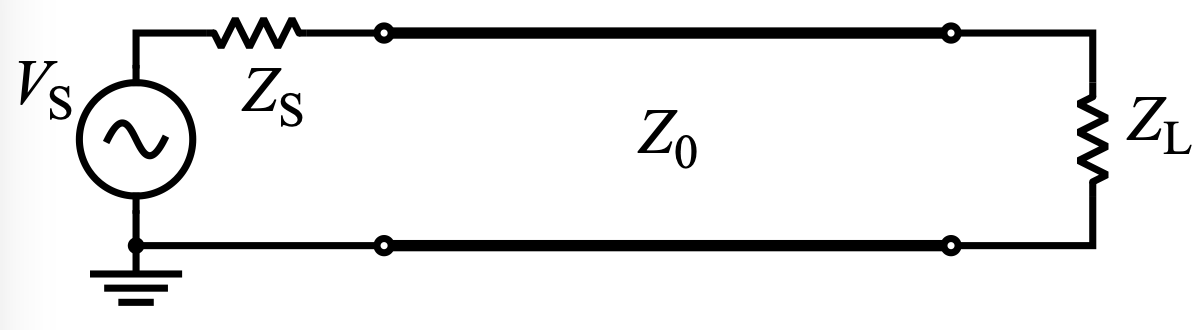
\includegraphics[width=0.9\linewidth]{imgs/tl_simple_schematic.png}
    \caption{Transmission Line Schematic. Adapted from \autocite{Wikipedia_2025_transmission_line}}
    \label{fig:tl-simple-schematic}
\end{figure}


In its simplest form, a transmission line consists of two conducting wires connected to a driving voltage and a load impedance as diagrammed in Figure \ref{fig:tl-simple-schematic}. The signal wire propagates the signal from the source to a load with impedance $Z_L$ and the other wire propagates the \emph{return signal} from the load back to the source. Ideally, the resistance of the transmission line will be zero so that the signal propagates losslessly. The wires generate magnetic fields as current flows through them due to their self-inductance while the capacitance between the wires couples the signals in them together. Instead of considering the inductance and capacitance of the line as a whole, a distributed element model can be employed using an inductance per unit length, $L$, in series and capacitance per unit length $C$ in parallel. Along a distance $dx$, we can then model the transmission line as in Figure \ref{fig:lc-base-unit}, so that the entire line consists of many repeating units of this circuit. 

\begin{figure}[h]
    \centering
    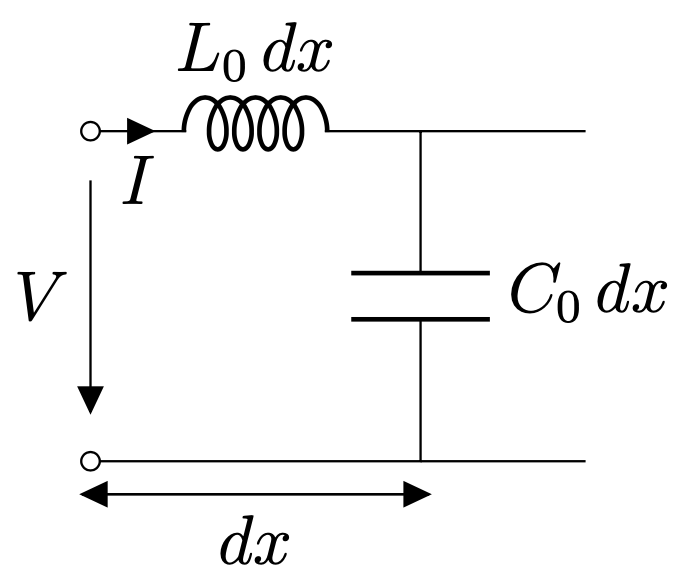
\includegraphics[width=0.4\linewidth]{imgs/lc_base_unit.png}
    \caption{Basic unit of lossless transmission line using distributed element model. Adapted from \autocite{UofT_PulsesInCables}}
    \label{fig:lc-base-unit}
\end{figure}

Using the governing equations for inductors and capacitors with the sign conventions in Figure \ref{fig:lc-base-unit}, we see that the change in voltage, $dV$, and current, $dI$, along length $dx$ in the transmission line follows
\begin{align}
    \label{eqn:dV_dx-telegraphers}
    \diffp{V}{x} &= -L\diffp{I}{t} \\ 
    \label{eqn:dI_dx-telegraphers}
    \diffp{I}{x} &= -C \diffp{V}{t}
\end{align}
where we `divided' $dV$ and $dI$ by $dx$ to obtain the partial derivatives. Substituting the equations into one another yields 
\begin{align}
    \label{eqn:V_wave_equation}
    \diffp[2]{V}{x} &= LC \diffp[2]{V}{t} \\ 
    \label{eqn:I_wave_equation}
    \diffp[2]{I}{x} &= LC \diffp[2]{I}{t} 
\end{align}
We recognize these as wave equations with general solutions
\begin{align}
    \label{eqn:v(x,t)-wave-solution}
    V(x,t) &= V_+(x - \nu t) + V_-(x + \nu t)\\ 
    \label{eqn:i(x,t)-wave-solution}
    I(x,t) &= I_+(x - \nu t) + I_-(x + \nu t)
\end{align}
where the $+$ subscript corresponds to forward traveling waves and the $-$ to reflected waves and $\nu$ is the propagation speed given by
\begin{equation}
    \label{eqn:nu(L0, C0)}
    \nu = \frac1{\sqrt{LC}}
\end{equation}

The initial conditions for the wave solutions are enforced by the driving signal from the voltage source. A "pulse" waveform consists of a square wave of some width sent intermittently at a set frequency. The width of the pulse is commensurate with the time it lasts via its propagation speed, so we can list the pulse width in time units. To see wave effects, we require pulses with widths much less than the length of the transmission line. 

As part of this investigation, we will examine how a discrete network of inductors and capacitors behaves as a transmission line by determining the propagation speed of a pulse through the circuit. The network consists of repeating units formed of an inductor with $L = (1.5 \pm 0.2)\,\mathrm{mH}$ and a capacitor with $C = (0.0100 \pm 0.0003)\,\mu\mathrm{F}$. The inductor is in series with the driving voltage and the capacitor parallel as in Figure \ref{fig:lc-base-unit}. Equation \ref{eqn:nu(L0, C0)} gives an expected propagation speed of 
\begin{equation}
    \label{eqn:nu(discrete-theoretical)}
    v = \ab(\frac{LC}{\unit{LCunit^2}})^{-1/2}\\ 
    = (0.26 \pm 0.01)\unit{\frac{LC unit}{ \micro s}}
\end{equation}
where an \unit{LC unit} is the length of 1 unit in the circuit. See Appendix Section \ref{appendix:propagation-speed-uncertainty} for the uncertainty calculation.

\subsection{Load Effect}
We demonstrate that the characteristic impedance of the transmission line,$Z_0$, and the load, $Z_L$, (see Figure \ref{fig:tl-simple-schematic}) characterize the reflection and transmission of waves in the line. 

Integrating Equation \ref{eqn:dV_dx-telegraphers} over length $dx$ using either the forward or reflected solutions for voltage and current in Equations \ref{eqn:v(x,t)-wave-solution} and \ref{eqn:i(x,t)-wave-solution} yields
\begin{equation}
    \label{eqn:v=vLi}
    V_{\pm} = \pm \nu L I_{\pm}
\end{equation}
The \emph{characteristic impedance} of the transmission line, $Z_0$, is then determined as
\begin{equation}
    \label{eqn:impedance=sqrt(L/C)}
    Z_0 = \frac{V_+}{I_+} = -\frac{V_-}{I_-} = \nu L = \sqrt{\frac{L}{C}}
\end{equation}
The load impedance satisfies $Z_L = V/I$ where $V$ and $I$ are as in Equations \ref{eqn:V_wave_equation} and \ref{eqn:I_wave_equation} with the arguments dropped for convenience. We can define reflection and transmission coefficients $r = V_-/V_+$ and $t = V/V_+$ respectively. Which can be expressed  
\begin{align}
    \label{eqn:r_reflection_coeff}
    r &= \frac{Z_L - Z_0}{Z_L + Z_0}\\ 
    \label{eqn:t_reflection_coeff}
    t &= \frac{2Z_0}{Z_L + Z_0}
\end{align}
An open circuit $(Z_L = \infty)$ then leads to $r = 1$ and $t = 0$ so that the entire wave is reflected so the average DC level is that of the driving signal. A short circuit $(Z_L = 0)$ gives $r = -1$ and $t$ undefined so that the wave is reflected with opposite amplitude and the average DC voltage is 0. In the context of pulses, we can consider the limiting case when the pulse widths are increased until they overlap to become a DC signal. For the short circuit case, there is no potential difference between the conducting lines, which matches the DC level being 0 on average. The open circuit drops the entire voltage before returning the signal, so the voltage difference is that of the driving source. For $Z_L = Z_0$, the reflected wave disappears in a process known as `impedance matching'. Conversely, any mismatch in impedance between the transmission line and a load will give rise to reflections. 

\subsection{Attenuation}
Real transmission lines have some finite resistance which diminishes the magnitude of the reflected wave. We express the attenuation of the signal in decibels as the ratio of the power of the initial voltage sent to the line, $V_i$, to the reflected voltage, $V_-$
\begin{equation}
    \label{eqn:attenuation-formula}
    \textrm{Attenuation} = 10\log_{10} \ab(\frac{V_-}{V_i})^2
\end{equation} 
We square the voltages since power is proportional to voltage squared. It should be noted that attenuation increases with cable length due to the increased resistance, and thus, is usually reported in $\unit{dB}$ per unit length. 

\subsection{Coaxial Cables}
Coaxial cables are a type of transmission line formed by two cylindrical conducting shells separated by a dielectric material as shown in Figure \ref{fig:coax-cross-section}. 

\begin{figure}[h]
    \centering
    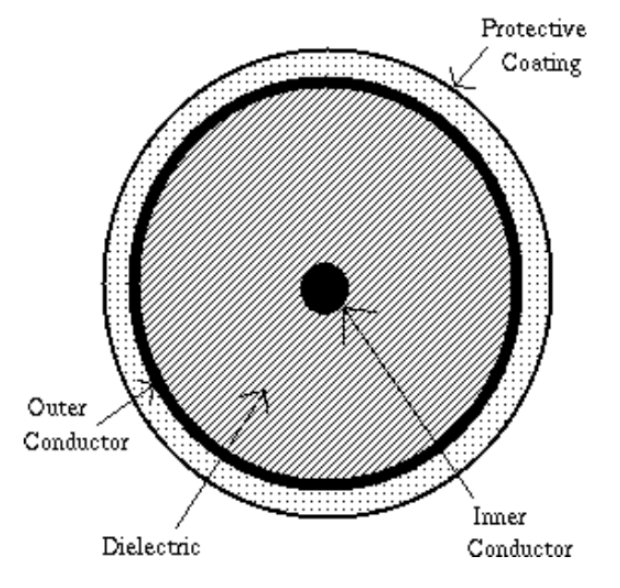
\includegraphics[width=0.5\linewidth]{imgs/coax_cross_section.png}
    \caption{Cross section of coaxial cable adapted from \autocite{UofT_PulsesInCables}}
    \label{fig:coax-cross-section}
\end{figure}
Let $R_1$ and $R_2$ denote the radii of the inner and outer conductors. Suppose some net charge $Q$ is distributed over the inner conductor with uniform density $Q/L$ where $L$ is the length of the transmission line. A cylindrical gaussian surface of length $\ell$ centered on the cable encloses charge $Q\ell/L$. Gauss's Law thus gives a radial electric field with magnitude 
\begin{equation}
    E(r) = \frac{Q/L}{2\pi r \e_0\e_r}, \qquad r \in [R_1, R_2]
\end{equation}
where $\e_0$ is the permittivity of free space and $\e_r$ is the relative permittivity of the dielectric. The voltage difference between the conductors is  
\begin{equation}
    V = \frac{Q/L}{2\pi\e_0\e_r}\int_{R_1}^{R_2} \frac{dr}{r} = \frac{Q/L}{2\pi \e_0\e_r} \ln\frac{R_2}{R_1}
\end{equation}
The capacitance per unit length of the cable is thus
\begin{equation}
\label{eqn:C0_coaxial}
    C = \frac{Q\ell/L}{V\ell} = \frac{2\pi \e_0 \e_r}{\ln \frac{R_2}{R_1}}
\end{equation}
For the inductance, suppose net current $I$ flows through the inner conductor. Then, Ampere's law gives an azimuthal magnetic field of magnitude 
\begin{equation}
    B = \frac{\mu_0\mu_r I}{2\pi r}, \qquad r \in [R_1, R_2] 
\end{equation}
where $\mu_0$ is the magnetic permeability of free space and $\mu_r$ is the relative permeability of the dielectric. The magnetic flux, $\Phi$, through a plane across the dielectric gap perpendicular to the cable axis with length $\ell$ is 
\begin{equation}
    \Phi = \frac{\mu_0\mu_r I \ell}{2\pi}\int_{R_1}^{R_2} \frac{dr}{r} = \frac{\mu_0\mu_r I \ell}{2\pi}\ln\frac{R_2}{R_1} 
\end{equation}
Hence, the inductance per unit length is
\begin{equation}
\label{eqn:I0_coaxial}
    L = \frac{\Phi}{I \ell} =  \frac{\mu_0\mu_r}{2\pi}\ln\frac{R_2}{R_1}
\end{equation}

From Equation \ref{eqn:nu(L0, C0)}, we find the speed of propagation in a coaxial cable to be 

\begin{equation}
    \label{eqn:nu(coaxial)}
    \nu = \frac1{\sqrt{\mu_0\mu_r\e_0\e_r}} = \frac{c}{\sqrt{\mu_r \e_r}} \approx \frac{c}{\sqrt{\e_r}}
\end{equation}
where $c$ is the speed of light and $c = 1/\sqrt{\e_0\mu_0}$. We also approximate $\mu_r \approx 1$ for standard dielectrics in coaxial cables like polyethylene \autocite{PHYS401Lecture04}. Using equation \ref{eqn:impedance=sqrt(L/C)}, we determine the characteristic impedance of the cable as 
\begin{align}
    Z_0 &= \frac1{2\pi}\sqrt{\frac{\mu_0\mu_r}{\e_0\e_r}} \ln \frac{R_2}{R_1} \\ 
    &\approx \frac{138}{\sqrt{\e_r}} \log_{10} \frac{R_2}{R_1}\\
    \label{eqn:impedance_coaxial}
    &= 138\frac{\nu}{c} \log_{10} \frac{R_2}{R_1} 
\end{align}
where we again approximated $\mu_r \approx 1$ and substituted Equation \ref{eqn:nu(coaxial)} in the last step. Thus, by measuring the speed of propagation of waves in a coaxial cable, we can determine characteristic impedance of the cable through \ref{eqn:impedance_coaxial} if its geometry is known.

Using this approach, we will determine the characteristic impedance of a coaxial BNC cable with a specified impedance of $50\Omega$. Further, we will see how the length of this BNC cable affects the attenuation of the signal. 

% In many introductory  courses, it is common to assume that any change in a circuit 
% instantaneously affects every component. In reality, electrical signals travel at finite 
% speeds determined by the physical properties of the cables and connectors used. When a 
% pulse is introduced into a cable, that pulse moves along the conductor according to wave-like 
% principles governed by the cable’s inductance and capacitance. These factors combine so that 
% the voltage and current in the line each satisfy a wave equation.

% To understand why pulses do not propagate instantaneously, consider that any cable can be 
% modeled as a continuous ladder of infinitesimally small inductors and capacitors. If $V$ is 
% the voltage at a point in the line and $I$ is the corresponding current, one finds through 
% basic circuit analysis that small elements of the cable store magnetic energy via inductance 
% and electric energy via capacitance, leading to coupled partial differential equations for 
% $V$ and $I$. Solving these equations yields wave equations of the general form 
% \[
% \frac{\partial^2 V}{\partial x^2} \;=\; L C\, \frac{\partial^2 V}{\partial t^2},
% \]
% where $L$ and $C$ denote the inductance and capacitance per unit length, respectively. 
% The key implication of these equations is that pulses have a finite propagation velocity 
% given by $\nu = 1/\sqrt{L C}$. For a typical coaxial cable, this velocity is somewhat 
% less than the speed of light $c$ because of the cable’s dielectric medium, whose permittivity 
% $\varepsilon$ and permeability $\mu$ determine exactly how quickly electromagnetic signals 
% can travel in the material.

% An important consequence of this wave-like behavior is that part or all of a pulse can 
% reflect at the end of a cable, depending on how the cable is terminated. This reflection 
% arises from boundary conditions: a cable of characteristic impedance $Z_0$ can only transmit 
% all of an incoming pulse if the load at its end has the same impedance. Otherwise, a reflected 
% pulse travels back up the cable in the negative direction. For instance, an open-circuited 
% cable (load impedance approaching infinity) sends back a pulse in the same orientation as 
% the incoming wave. By contrast, a short-circuited end inverts the pulse upon reflection 
% because the boundary forces the voltage to be zero at that point. Mathematically, one 
% describes this effect using the reflection coefficient
% \[
% r = \frac{Z_L - Z_0}{Z_L + Z_0},
% \]
% where $Z_L$ is the load impedance. If $Z_L$ equals the characteristic impedance $Z_0$, then 
% $r = 0$ and there is no reflection, behaving like an infinitely long, lossless line.

% From a fundamental physics standpoint, the characteristic impedance $Z_0$ captures how 
% voltage and current relate in a traveling wave, and it can be derived from the ratio of 
% voltage to current in the wave solutions. In other words, $Z_0 = \sqrt{L / C}$ in an 
% ideal cable with purely real inductance and capacitance. Real cables also exhibit resistive 
% and other dissipative effects, but the essential wave-like features remain clear as long as 
% pulses are short enough in duration to highlight travel times, reflections, and any resulting 
% attenuation. Because these effects depend strongly on the dielectric within the cable, 
% measurable quantities such as signal speed and attenuation are pivotal when designing or 
% analyzing high-frequency circuits, communication lines, or pulse-based measurements.


\section{Methods and Procedures}
The experiment was conducted to study pulse propagation in transmission lines and coaxial cables. A KEYSIGHT EDU33211A waveform generator was utilized to produce electrical pulses, and these pulses were measured using a KEYSIGHT DSOX1202G digital oscilloscope. Both devices were connected via a TEE connector, with a transmission line connected to the open arm of the TEE connector as shown in Figure \ref{fig:exp_setup_diagram}. 
\begin{figure}[h]
    \centering
    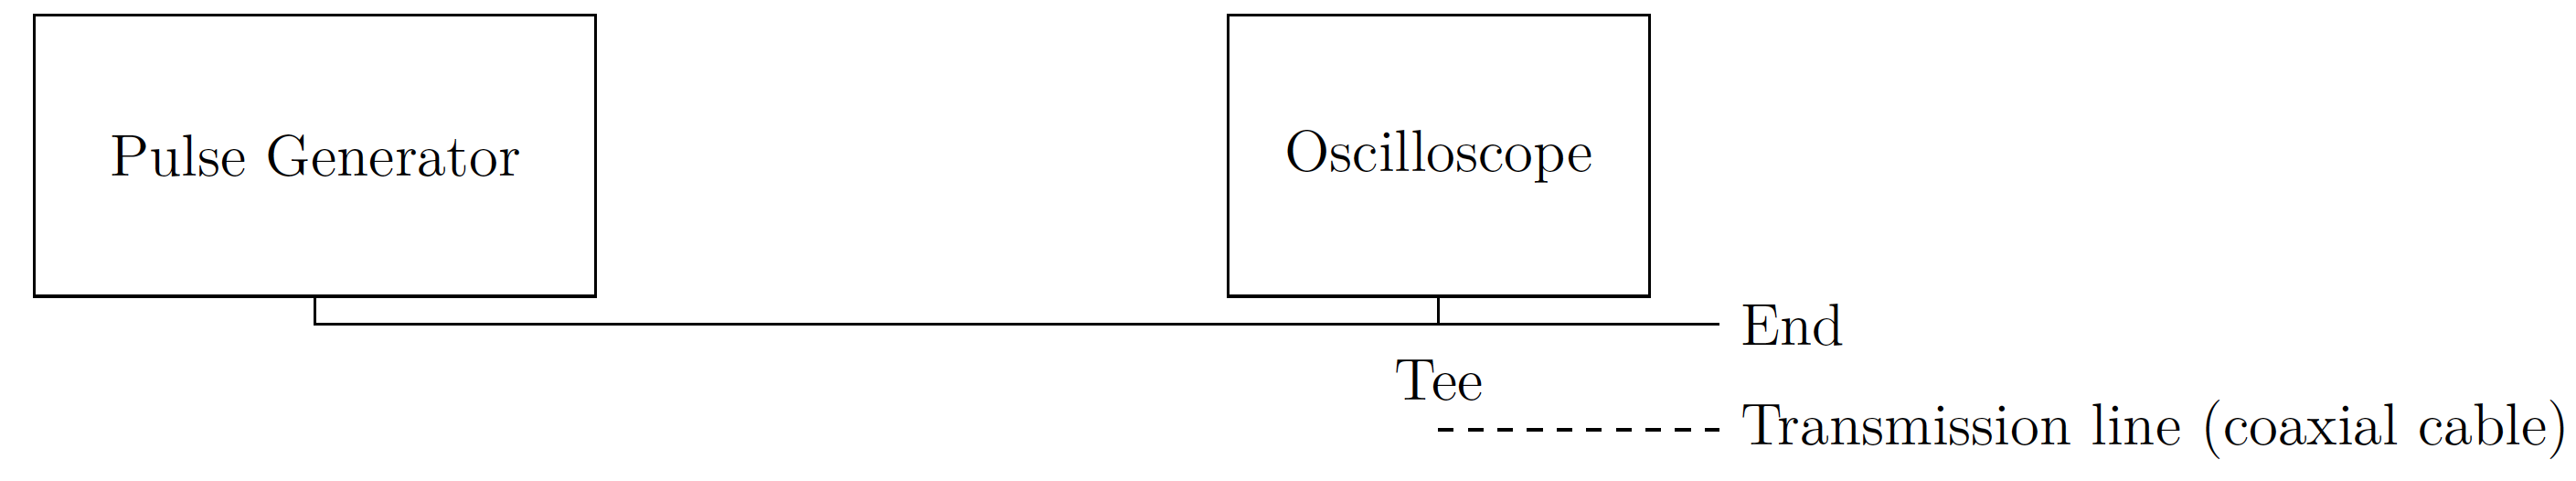
\includegraphics[width=0.99\linewidth]{imgs/Screen Shot 2025-03-27 at 11.48.26 PM.png}
    \caption{Schematic of the experimental setup used to investigate pulse propagation 
    and reflections in a coaxial transmission line.}
    \label{fig:exp_setup_diagram}
\end{figure}


Initially, a transmission line composed of 41 LC (inductor-capacitor) units, each consisting of a $(0.0100 \pm 0.0003)$ µF capacitor and a $(1.5 \pm 0.2)$ mH inductor, was connected to the TEE connector. The far end of the transmission line was connected directly to channel 2 of the oscilloscope. Pulses with an initial width of approximately 75 µs and a frequency around 300 Hz were generated. Where we observed clear reflected and transmitted pulses on channel 1 and 2 respectively.

With this setup, channel 1 of the oscilloscope observes the reflected pulse while channel 2 sees the transmitted. However, since the impedance of this LC unit model is not equal to that of the connecting cables, additional reflections are present on both channels. To reduce these, a variable resistor was connected across the end of the transmission line, and the resistance was adjusted until these additional pulses were neutralized. The delay time between channels 1 and 2 was then recorded using the oscilloscope measure functionality as the number of LC units in the transmission model was varied from 41 to 32. 

Another set of experiments were conducted with 50 $\Omega$ coaxial cables (Belden product 8259 \autocite{Belden8259_BNC_Datasheet}). These cables have a polyethylene insulation so that $\mu_r = 1$ and $\e_r = 2.25$ \autocite{UofT_PulsesInCables}. Further, the inner conductor diameter is specified as $0.035\unit{in}$ while the outer shield has diameter $0.117\unit{in}$ \autocite{Belden8259_BNC_Datasheet}. We had access to 3 unique cables of lengths $(15.09 \pm 0.02)\unit{m}, (30.50\pm0.05)\unit{m}$ and $(75.84 \pm 0.02)\unit{m}$. 

With the waveform generator TEE'd to a channel on the oscilloscope, one of the coaxial cables was attached to the other end of the TEE. The end of the coaxial cable was left open so that the pulse would be reflected entirely according to Equation \ref{eqn:r_reflection_coeff} and the attenuation of the signal could be measured. The waveform generator was configured with a peak-to-peak voltage of $4\unit{V}$, 50$\unit{ns}$ width, and frequency $15 \unit{kHz}$. With the oscilloscope horizontal and vertical scales adjusted to $2\unit{V/div}$ and $500\unit{ns/div}$ respectively, we were able to observe a time series of the initial pulse followed by a reflected pulse. This time series was recorded using the 3 cables on their own and then every combination of 2 cables from the 3 were joined using a BNC connector to obtain 3 additional effective cable lengths. Since the BNC connector had length less than the uncertainty in the cable lengths themselves, it was considered negligible. 

%Pulse delay times were measured and compared against expected propagation times based on the dielectric constant of the cable insulator. The attenuation of the cables was also assessed by analyzing reflected pulses from an open-circuit termination, quantified in decibels per meter (dB/m). Characteristic impedance values for the coaxial cable were derived experimentally from observed reflections.






\section{Analysis and Discussion}
\subsection{Discrete LC unit Network}
\begin{figure}[h]
    \centering
    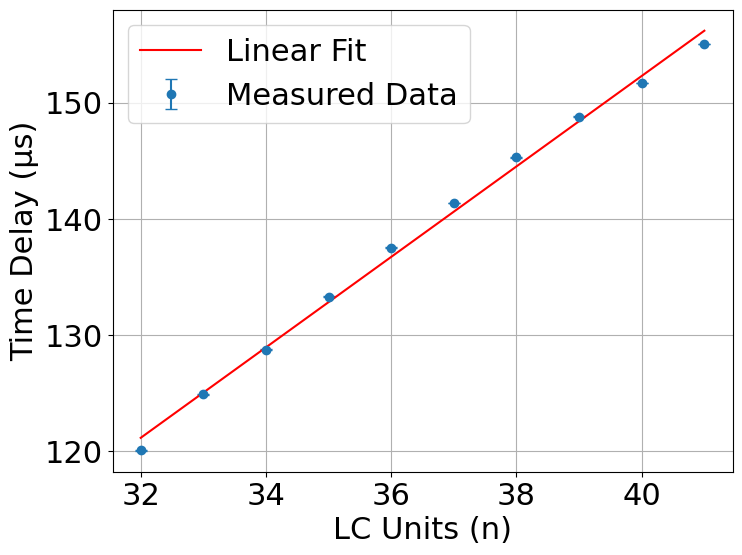
\includegraphics[width=0.8\linewidth]{imgs/time.png}
        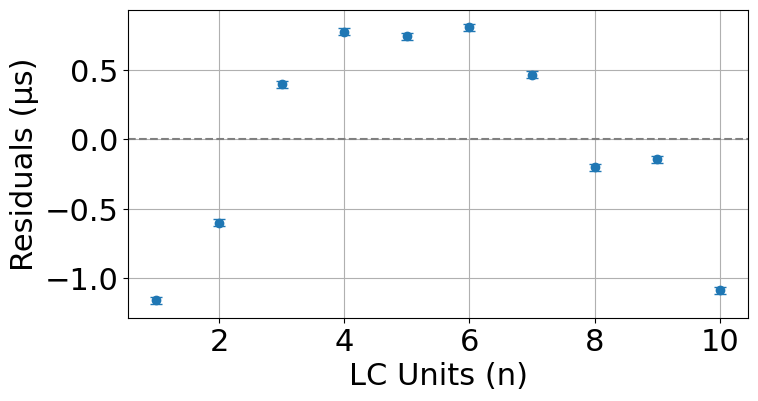
\includegraphics[width=0.8\linewidth]{imgs/residuals.png}
\caption{(Top) Time delay versus the number of LC units (blue circles), measured using pulses with a width of approximately 75~$\mu$s generated at 300~Hz, shown with the best-fit line $\Delta t(n) = m\,n + b$. The linear regression yields $m \approx 3.9 \pm 0.1\,\mu\text{s/LC unit}$ and $b \approx -4 \pm 2\,\mu\text{s}$, with a large reduced chi-squared ($\chi^2_{\mathrm{red}} = 1021$) and a chi-squared probability of zero ($\chi^2_{\mathrm{prob}}=0$). (Bottom) Residual analysis of the linear fit. Residuals show a clear systematic deviation from random scatter. Error bars too small to see, but in both represent the oscilloscope time-base uncertainty.}

    \label{fig:timedelay}
\end{figure}
In this experiment, we investigated how pulses travel through a discrete ``transmission line'' made up of multiple LC units, each composed of a capacitor and an inductor. We used a function generator to inject square pulses into one end of the LC line and measured how the overall pulse delay changed when we varied the number of these LC units. Since each section has an inductance of $L = 1.5 \pm 0.2\,\mathrm{mH}$  and a capacitance of $C = 0.0100 \pm 0.0003\unit{\micro F}$, we expected the total delay to scale linearly with the number of sections through Equation \ref{eqn:nu(L0, C0)} with an expected speed of $(0.26 \pm 0.01)\unit{LCunit/\micro s}$ as shown in Equation \ref{eqn:nu(discrete-theoretical)}.  

The raw data \ref{tab:lcdata} we acquired consisted of time-delay measurements for integers of LC units ranging primarily from 32 to 41 units. Our plan for analyzing these measurements was straightforward: we plotted time delay against the number of LC units (Figure \ref{fig:timedelay}), fit a straight line to those data points, and determined the slope and intercept of that line. The slope provides direct insight into how much time delay each LC section contributes. By taking the reciprocal of that slope, we obtain a measured propagation speed in ``LC units per microsecond.'' We used this linear-fit approach because theory predicts that each LC section should contribute the same incremental delay, making a constant-slope trend likely. If the results had displayed large curvature or systematic trends in the residuals, we would have considered higher-order or more intricate fits, but the linear model is strongly motivated by the standard wave equation for transmission lines.

Our linear regression (Figure \ref{fig:timedelay}) yielded a slope of  $3.9 \pm 0.1\,\mu\mathrm{s}$ per LC unit, which implies an experimental speed of 
\[
v_{\mathrm{exp}} \;=\; \frac{1}{\text{slope}} \;=\; 0.26\,\pm\,0.01 \unit{LCunit/\micro s}
\]
The residuals \ref{fig:timedelay} show a systematic pattern rather than random scatter: they begin negative, rise to positive values towards the middle and slightly right of the plot, and then decrease again. This pattern suggests a deviation from the linear model, indicating the possibility of underlying effects or measurement issues not captured by the simple linear relationship.

The experimental value of $0.26,\pm\,0.01\;\mathrm{LC\;units/\mu s}$ agrees extremely well with the theoretical prediction, as the two values differ by only $0.61\%$.\footnote{The percent error calculation was performed using exact numerical values before rounding for significant figures, not the rounded values presented here.} This level of agreement is well within the uncertainties for both the measurement and the component tolerances, so we can conclude that our data validate the expected relationship.

The statistical analysis of the linear regression provides insight into the quality of our fit. The high chi-square value ($\chi^2 = 8172$) with 8 degrees of freedom leads to an excessively large reduced chi-squared value ($\chi^2_{\mathrm{red}} = 1021$) and a corresponding chi-squared probability ($\chi^2_{\mathrm{prob}} = 0$). This probability indicates that, statistically, the fit is extremely unlikely to represent the data accurately given the stated uncertainties. Such a large reduced chi-squared value suggests that the residuals exceed the uncertainties accounted for by the oscilloscope’s time-base resolution (0.025~$\mu$s), pointing toward additional systematic uncertainties or experimental factors not captured by the instrument's resolution alone.

This discrepancy shows that the uncertainty in our measurements is likely larger than the experimental uncertainty alone. In addition to inherent instrument resolution and component tolerances, factors such as signal distortion make it more challenging to determine the exact time delay. This, combined with extra wiring capacitance, resistance in the connectors, and  variations in the LC components, contributes to a systematic error that is not captured by the oscilloscope's time-base uncertainty. Overall, the strong linear correlation and the excellent agreement between the experimental and theoretical propagation speeds confirm that each LC section contributes nearly the same incremental time delay. Nonetheless, the large reduced chi-squared highlights that the effective uncertainties are larger than what the oscilloscope’s settings suggest.
 
One of the most important sources of uncertainty in our measurements involved the rated tolerances of the LC components themselves. Because the propagation speed depends on $1/\sqrt{L\,C}$, a relatively small variation in either inductance or capacitance can shift the theoretical speed by a noticeable fraction.








\subsection{Coaxial Analysis}
\subsubsection{Characteristic Impedance}
We seek to determine the characteristic impedance of a 50$\Omega$ BNC cable experimentally. For each cable length tested, we determine the delay between the initial and reflected pulse by taking the difference in time between the locations of the 2 peaks in the time series data (see Figure \ref{fig:coaxial-time-series} in the Appendix). Some smaller peaks were observed in the time series, however, they were significantly smaller than the initial and reflected pulses and were ignored in the analysis. The delay between the two peaks corresponds to the pulse traveling the length of the cable and back, so we halve it to get the true propagation time. Using this, we can obtain the propagation speed of the pulse through a linear fit which yields the permittivity of the dielectric through Equation \ref{eqn:nu(coaxial)} and subsequently the impedance through Equation \ref{eqn:impedance_coaxial}. 

\begin{figure}[h]
    \centering
    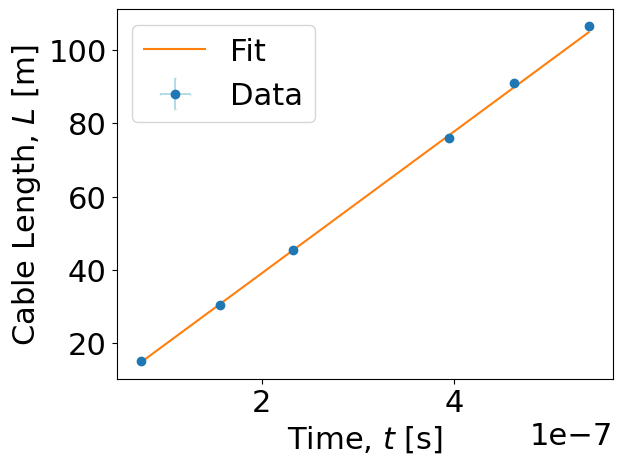
\includegraphics[width=0.8\linewidth]{imgs/delay_coaxial.png}
    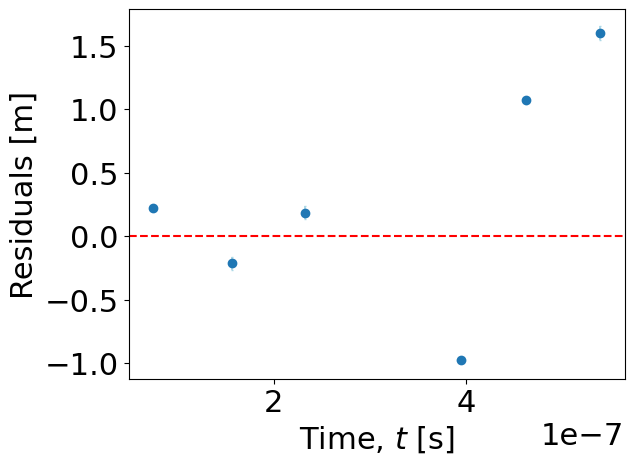
\includegraphics[width=0.8\linewidth]{imgs/delay_coaxial_res.png}
    \caption{(Top) Propagation times for pulse in BNC cable with $4\unit{V}$ peak-to-peak voltage, 50$\unit{ns}$ width, and $15\unit{kHz}$ frequency for various cable lengths. Error bars too small to see. Length plotted against propagation time with linear fit yielding propagation speed of $\nu = (193.28 \pm 0.07)\unit{m/\micro s}$ with offset $(0.47 \pm 0.02)\unit{m}$. Fit achieves $\chi^2_{red} = 1209$ and $\chi^2_{prob} = 0$. (Bottom) Residuals of fit}
    \label{fig:coaxial_delay}
\end{figure}

Figure \ref{fig:coaxial_delay} showcases a positive trend in the cable length versus propagation time. The linear fit gives a speed of $\nu = (193.28 \pm 0.07)\unit{m/\micro s}$ but performs poorly with $\chi^2_{red} = 1209$ and $\chi^2_{prob} = 0$ due to the smallness of the errorbars. 

We observe that the propagation speed is reduced from the speed of light by a factor of $\sqrt{\e_r}$ as per Equation \ref{eqn:nu(coaxial)}. We thus determine $\e_r = 2.410 \pm 0.002$ which is larger than the expected value of $2.25$. 

Using the experimental permittivity, we find the characteristic impedance of the cable to be $Z_0 = 138/\sqrt{e_r} \log_{10}(0.117/0.035) = (46.60 \pm 0.02)\Omega$ using the diameters listed in \autocite{Belden8259_BNC_Datasheet}. The result is in good alignment with the specified rating of $50\Omega$ with a $6.8\%$ percent error. This also supports the observation of the reflected pulse diminishing almost completely with the addition of a a 51$\Omega$ termination to the cable.

The inductance of the line may have been increased due to the cable being looped to fit on the table. This would lead to a smaller propagation speed due to Equation \ref{eqn:nu(L0, C0)} which produces a larger permittivity from Equation \ref{eqn:nu(coaxial)} and consequently a smaller impedance. Future experiments should investigate the extent to which cable loops affect this result. The contribution could be mitigated by laying out the cable without any loops. 
From the residuals in Figure \ref{fig:coaxial_delay}, we see that the linear fit performs worse for the 3 largest cable lengths. These lengths were composed of 2 connected cables which may have introduced additional distortions in the signal which was not accounted for in the analysis. The poorness of the fit suggests the need for a more robust method to determine the time delay of the pulses. The reflected pulse was observed to be distorted due to the attenuation from the cable as seen in the time series in Figure \ref{fig:coaxial-time-series}. The delay between the transmitted and reflected pulses may be better measured using the onset of each pulse instead of their peaks as the peak can shift from the pulse onset due to distortion. Alternatively, higher quality cables with lower signal loss could be used to reduce the distortion in the reflected pulse so that the time delay could be better measured.

\subsubsection{Attenuation}
We also aim to determine the attenuation of the coaxial cable using the same time series data as in the impedance analysis. For each cable length, we find the attenuation by comparing the size of the transmitted and reflected pulse then applying Equation \ref{eqn:attenuation-formula}. We can then determine the attenuation per unit length of the cable. The size of each pulse is estimated as the peak voltage of the pulse subtracted by the baseline reading (average of pre-pulse region) in the time series. Figure \ref{fig:attenuation_coaxial} plots these attenuations against cable length, and a linear fit yields an attenuation of $(-0.05 \pm 0.02)\unit{dB/m}$ with $\chi^2_{red} = 0.03$ and $\chi^2_{prob} = 0.99$. The fit statistics are inflated due to the large relative errors on the attenuations. These propagate from the uncertainties in the voltage readings of the oscilloscope which have a minimum $3\%$ error \autocite{KeysightOscopeDatasheet}. Better results could be achieved with a higher accuracy voltage reading of the signal. 

\begin{figure}[h]
    \centering
    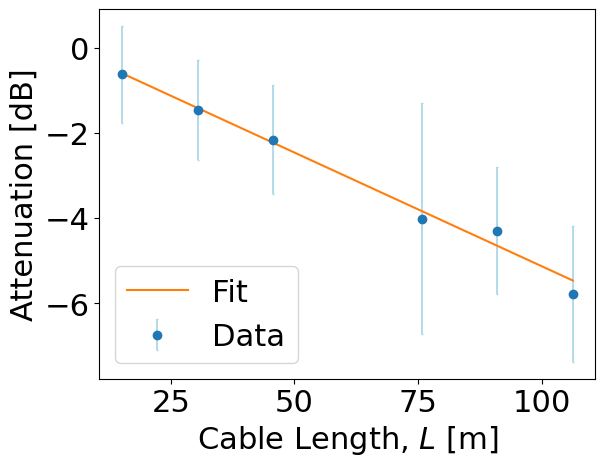
\includegraphics[width=0.8\linewidth]{imgs/attenuation_coaxial.png}
    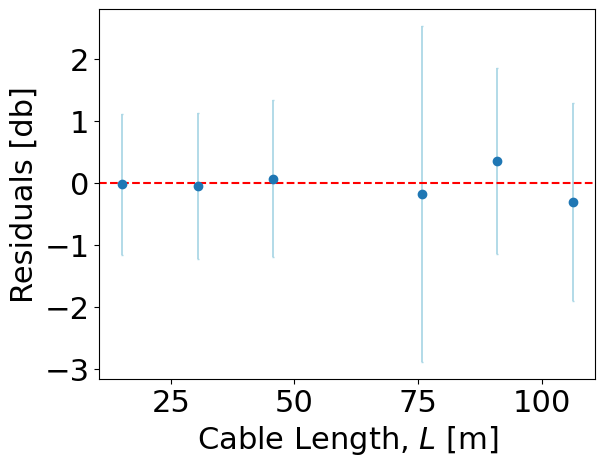
\includegraphics[width=0.8\linewidth]{imgs/attenuation_coaxial_res.png}
    \caption{(Top) Attenuation of signal in BNC cable of various lengths driven by pulse with $4\unit{V}$ peak-to-peak voltage, 50$\unit{ns}$ width and $15\unit{kHz}$ frequency. Linear fit applied with parameters $(-0.05 \pm 0.02)\unit{dB/m}$ and $(0 \pm 1)\unit{dB}$. Fit achieves $\chi^2_{red} = 0.03$ and $\chi^2_{prob} = 0.99$. (Bottom) Residuals of fit.}
    \label{fig:attenuation_coaxial}
\end{figure}


\section{Conclusion}
We investigated the behavior of pulses generated by a KEYSIGHT EDU33211A waveform generator in 2 separate transmission lines as measured by a KEYSIGHT DSOX1202G oscilloscope. The first transmission line was composed of a discrete network composed of repeating LC (inductor-capacitor) units, each with $(0.0100 \pm 0.0003)$ µF capacitor and a $(1.5 \pm 0.2)$ mH inductor. The number of units was varied from 41 to 32 and the delay between the transmitted and reflected pulse on the two channels of the oscilloscope was measured to give the propagation speed of the wave. 
%\textbf{TOODOOO} add results with goodness of fits and how it compares with expected 
The linear fit of the measured data yielded a large chi-squared value of $\chi^2 = 8172$ with 8 degrees of freedom, corresponding to a very large reduced chi-squared of $\chi^2_{\mathrm{red}} = 1021$ and a chi-squared probability of $\chi^2_{\mathrm{prob}} = 0$. This low chi-squared probability indicates that the uncertainties considered (oscilloscope time-base uncertainty of $0.025\,\mu$s) significantly underestimate the true uncertainty, this suggests that the uncertainties in our measurements were significantly underestimated or that the model did not fully capture all experimental factors.

Coaxial BNC cables (Belden product 8259) were then used as transmission lines with driving pulses of $4\unit{V}$ peak-to-peak voltage, 50$\unit{ns}$ width, and $15\unit{kHz}$. 3 unique lengths of cables were attached to the oscilloscope via a TEE connector with the other ends of the TEE connected to the waveform generator and the oscilloscope. The other end of the cable was left open so that incoming pulses would be entirely reflected. 3 other lengths were tested by joining combinations of 2 cables. Time delays were obtained by comparing the delay between the peaks of the initial and reflected pulse. Halving this producing the propagation time of the signal. Plotting this against cable length produced Figure \ref{fig:coaxial_delay} and a linear fit produced a propagation speed of $\nu = (193.28 \pm 0.07)\unit{m/\micro s}$ which is reduced from the speed of light by $\sqrt{\e_r}$ as shown in Equation \ref{eqn:nu(coaxial)}. From this, we determined the permittivity of the dielectric in the cable to be $(2.410 \pm 0.002)$, overestimating the 2.25 permittivity of polyethylene. We found the characteristic impedance of the cable to be $(46.60 \pm 0.02)\Omega$ through Equation \ref{eqn:impedance_coaxial}, undershooting the specified rating of $50\Omega$. These deviations could be explained by the additional inductance of the cable due to looping. Future experiments should account for this impedance or mitigate it by laying the cable out flat. The fit performed poorly with $\chi^2_{red} = 1209$ and $\chi^2_{prob} = 0$ due to the smallness of the errorbars which calls for a better measurement of the time delay. This could be obtained by using cables with lower loss characteristics so that the reflected signal is less distorted. Residuals in the linear fit were seen to increase for the data taken with the joined cables, indicating that the BNC connector may have introduced additional distortion in the signal making the time delay estimation less certain.

The attenuation of the signal was measured for the various cable lengths by comparing the size of the initial and reflected pulses. The attenuation is plotted against cable length in Figure \ref{fig:attenuation_coaxial} and a linear fit yields an attenuation of $(-0.05 \pm 0.02)\unit{dB/m}$. The fit achieves $\chi^2_{prob} = 1$ due to the largeness of the errorbars which stem from the large relative uncertainty in the oscilloscope voltage readings. Better attenuation measurements require a more precise voltage reading. 





%	 REFERENCES
%----------------------------------------------------------------------------------------

\printbibliography % Output the bibliography


%----------------------------------------------------------------------------------------

\newpage

\appendix
\section*{Appendix}
\renewcommand{\thesubsection}{\Roman{subsection}}
\textbf{Statement of AI Usage} Used Vscode automatic code suggestions from Github Copilot and Coedeium during analysis to help write out functions and debug. 

\subsection{Propagation Speed Uncertainty}
\label{appendix:propagation-speed-uncertainty}
If a discrete transmission line is described by inductance $L$ and capacitance $C$ per section, 
its propagation speed is 
\[
v \;=\; \frac{1}{\sqrt{L\,C}}.
\]
Treating $L$ and $C$ as independent variables with small uncertainties $\Delta L$ and $\Delta C$, 
we note that 
\[
\ln v 
\;=\; 
-\tfrac12 \ln(L\,C)
\quad\Longrightarrow\quad
\frac{d v}{v} 
\;=\; 
-\tfrac12 
\Bigl(
\frac{dL}{L} 
+ 
\frac{dC}{C}
\Bigr).
\]
uncertainty becomes
\[
\Bigl(\frac{\Delta v}{v}\Bigr)^2
\;=\;
\tfrac{1}{4}
\Bigl[
\Bigl(\tfrac{\Delta L}{L}\Bigr)^2
+
\Bigl(\tfrac{\Delta C}{C}\Bigr)^2
\Bigr],
\]
leading to
\[
\frac{\Delta v}{v}
\;=\;
\tfrac12
\sqrt{
\Bigl(\tfrac{\Delta L}{L}\Bigr)^2
+
\Bigl(\tfrac{\Delta C}{C}\Bigr)^2
}.
\]
Multiplying by $v$ 
\[
\Delta v
\;=\;
v \;\times\;
\tfrac12
\sqrt{
\Bigl(\tfrac{\Delta L}{L}\Bigr)^2
+
\Bigl(\tfrac{\Delta C}{C}\Bigr)^2
}.
\]
Hence 
\[
v_{\mathrm{theoretical}} = \frac{1}{\sqrt{L\,C}},
\]
the total uncertainty is 
\[
\Delta v_{\mathrm{theoretical}}
\;=\;
v_{\mathrm{theoretical}}
\;\times\;
\frac12
\sqrt{
\Bigl(\tfrac{\Delta L}{L}\Bigr)^2
+
\Bigl(\tfrac{\Delta C}{C}\Bigr)^2
}.
\]

\subsection{Supplementary Tables and Figures}
\label{appendix:supp-figs}
\begin{table}[h]
\centering
\caption{Measured time delay for pulse propagation through varying numbers of LC units. The table lists the number of LC units in the discrete transmission line network and the corresponding measured pulse delay times. These delays were recorded using an oscilloscope with a time-base uncertainty of $\pm 0.025\,\mu$s, derived from the oscilloscope resolution of $500\,\text{ns/div}$ across $10$ divisions. Each LC unit consists of a capacitor ($C = 0.0100 \pm 0.0003\,\mu\text{F}$) and an inductor ($L = 1.5 \pm 0.2\,\text{mH}$).}
\label{tab:lcdata}
\begin{tabular}{c c}
\hline
\textbf{LC Units (n)} & \textbf{Time Delay ($\mu$s)} \\
\hline
41 & 155.04 \\
40 & 151.70 \\
39 & 148.80 \\
38 & 145.28 \\
37 & 141.35 \\
36 & 137.52 \\
35 & 133.28 \\
34 & 128.72 \\
33 & 124.88 \\
32 & 120.04 \\
\hline
\end{tabular}
\end{table}


\begin{figure}[h]
    \centering
    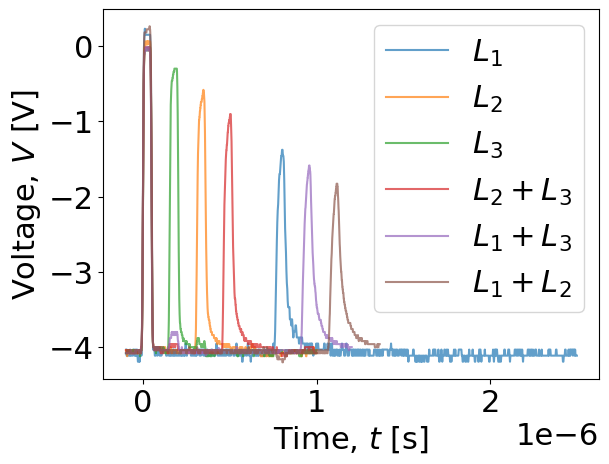
\includegraphics[width=0.99\linewidth]{imgs/coaxial_time_series.png}
    \caption{Raw time series for Keysight oscilloscope measurements of voltage in open-ended BNC cable driven by pulse as diagrammed in Figure \ref{fig:exp_setup_diagram}. Pulse configured with $4\unit{V}$ peak-to-peak voltage, 50$\unit{ns}$ width, and $15\unit{kHz}$ frequency over various cable lengths. $L_1 = (15.09 \pm 0.02)\unit{m}, L_2 = (30.50\pm0.05)\unit{m}$ and $L_3 = (75.84 \pm 0.02)\unit{m}$.}
    \label{fig:coaxial-time-series}
\end{figure}

\end{document}
